\ifslide{
  \section[Agenda]{}

  \setcounter{tocdepth}{2}

  \begin{frame}
    \begin{multicols}{2}
      \fontsize{7}{8}{
        \tableofcontents[part=1]

      }
    \end{multicols}
  \end{frame}
  \part{Introduction au Middleware}
}

\ifbook{
  \chapter{Le Middleware}
}

\section{A - Rappel} % (09/01/2012)}

\mysubsection{Fonctionnement d'un ordinateur}

\ifbook{

  \mysubsubsection{Fonctionnement schématique d'un ordinateur}

  \paragraph{} Avant d'entrer dans le coeur du sujet, il est nécessaire de tout d'abord bien
  comprendre comment fonctionne la brique la plus élémentaire de tout système informatique:
  l'ordinateur.

  \begin{figure}[hb]
    \begin{center}
      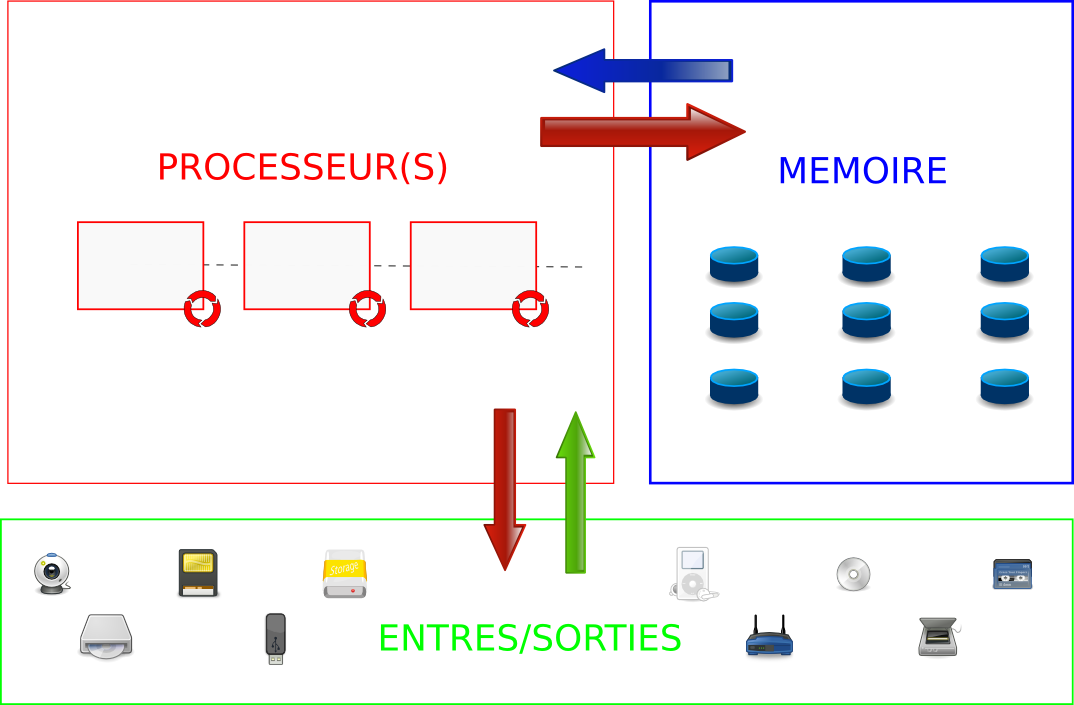
\includegraphics[scale=0.3]{img/cpu-schematics.png}
      \caption{Schéma simplifié du fonctionnement d'un ordinateur}
      \label{schema-ordi}
    \end{center}
  \end{figure}

  \paragraph{} Comme l'illustre le dessin \ref{schema-ordi} (page \pageref{schema-ordi}), un
  ordinateur, aussi complexe soit-il peut être résumé aux trois composants suivants:
  \begin{description}
    \item[Processeur] unité de traitement de l'ordinateur, c'est lui qui réalise les calculs et qui
    produit les résultats ;
    \item[Mémoire] espace de travail du processeur, la mémoire lui permet de stocker les résultats,
    intermédiaires ou finaux, de ses calculs ;
    \item[Entrées/Sorties] pour communiquer avec le "monde extérieur" (clavier, écran, disques durs,
    réseaux,...) le processeur dispose de différents composants matériels dédiés aux différentes
    entrées/sorties.
  \end{description}

  \paragraph{Distinction mémoire vive et mémoire morte} Sans rentrer dans les détails techniques, il
  est important de noter que les périphériques de stockage, tels que les disques durs, ne sont pas
  conceptuellement très différents de la mémoire. Dans les deux cas, ils permettent au processeur de
  stocker des résultats.

  \paragraph{Distinction des types de mémoires} Il existe différents types de mémoires qui peuvent
  être séparées selon qu'elles sont rapide ou lente : plus la mémoire est "proche" du processeur,
  plus elle est rapide. Nous avons donc par ordre décroissant de vitesse :

  \begin{itemize}
    \item la RAM,
    \item le disque dur,
    \item le stockage sur une machine distincte.
  \end{itemize}

  \paragraph{Distinction mémoire vive et mémoire morte}  En outre, il faut noter qu'une mémoire
  \textbf{volatile} a besoin d'électricité pour être conservée, à la différence du \textbf{stockage
  de masse} qui lui conserver l'information une fois l'alimentation coupé. La mémoire volatile est
 donc perdu à chaque arrêt d'un ordinateur alors que les données placées dans la mémoire de masse
 sont conservés..

  \paragraph{} La mémoire vive d'un ordinateur (la "RAM") est une mémoire volatile, et les disques
  dur sont des mémoires de masse.

  \paragraph{} Ce qui sépare donc ces deux composants est leur \textbf{persistance}. L'information
  située en mémoire dite vive (comme la RAM) est \textbf{volatile} : elle disparaît si l'ordinateur s'éteint brusquement. À
  l'inverse, les données placées sur un périphérique de stockage, persiste au delà de l'extinction de
  l'ordinateur.
}

\ifslide{
  \begin{frame}{Qu'est-ce qu'un ordinateur ?}
   \begin{center}
     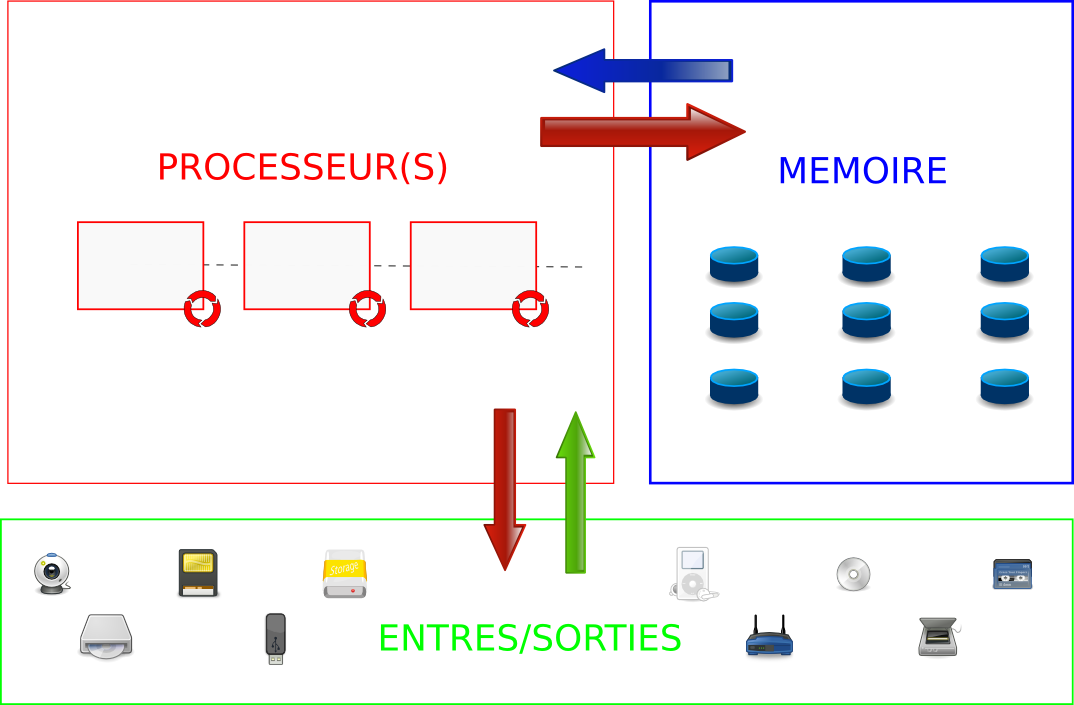
\includegraphics[scale=0.3]{img/cpu-schematics.png}
   \end{center}
  \end{frame}
}

\ifbook{
    \mysubsubsection{Rôle du système d'exploitation}

    \paragraph{} Encore une fois de manière très schématique, et surtout en restant pertinent par
    rapport au thème du cours, le \textit{Middleware}, nous allons maintenant brièvement évoquer le
    rôle du système d'exploitation.

    \paragraph{} En repartant de ce que nous venons de détailler sur le fonctionnement d'un
    ordinateur, plusieurs points peuvent rapidement être gênants. Le principal est que le processeur
    n'exécute qu'un seul programme à la fois, donc tel quel, une seule application peut s'exécuter
    sur un ordinateur à la fois.

    \paragraph{} Le système d'exploitation est une couche logicielle qui va permettre aux programmes
    s'exécutant sur l'ordinateur de se partager les ressources mises à disposition par l'ordinateur
    (processeur, mémoire, périphériques de stockage,...). En outre, le système d'exploitation va
    jouer le rôle d'arbitre entre ces différents programmes, leur attribuant chacun à leur tour un
    certain temps d'utilisation de ces ressources.

    \paragraph{} Ainsi, c'est grâce aux systèmes d'exploitation que de multiples programmes vont
    pouvoir s'exécuter en \textbf{parallèle} sur une machine, qu'elle possède un ou plusieurs
    processeurs.

    \paragraph{} Il est important de noter qu'aucun ordinateur ne pourra effectuer plus de tâches en
    parallèle que son nombre de processeurs, mais les cycles d'exécutions étant extrêmement courts,
    un seul ordinateur, équipé d'un seul processeur, peut donner l'impression à son utilisateur
    d'exécuter simultanément plusieurs tâches. C'est l'impression que vous donne tous les jours,
    les ordinateurs dédiés à la bureautique que vous utilisez.

    \paragraph{Remarque} On notera aussi au passage qu'un même programme peut lui même se diviser en
    plusieurs processus distincts, s'exécutant aussi en parallèle, selon les règles évoquées juste
    avant. Ainsi, dans la cadre d'un projet \textit{middleware} la question de l'exécution, de
    manière concurrente, de différentes parties de l'application peut se poser... (Nous y
    reviendrons plus loin dans le cours).

    \paragraph{} Le schéma \ref{role-os} (page \pageref{role-os} résume les principales
    fonctionnalités d'un système d'exploitation vis-à-vis des applications qui s'exécutent en son
    sein.

    \begin{figure}[h]
      \begin{center}
        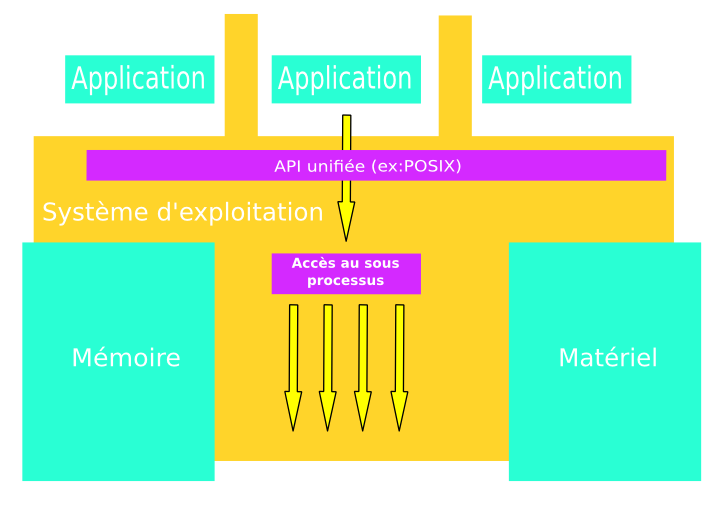
\includegraphics[scale=0.3]{img/operating-system.png}
        \caption{Rôle du système d'exploitation}
        \label{role-os}
      \end{center}
    \end{figure}
}

\ifslide{
  \begin{frame}{Le rôle du système d'exploitation}
    \begin{center}
      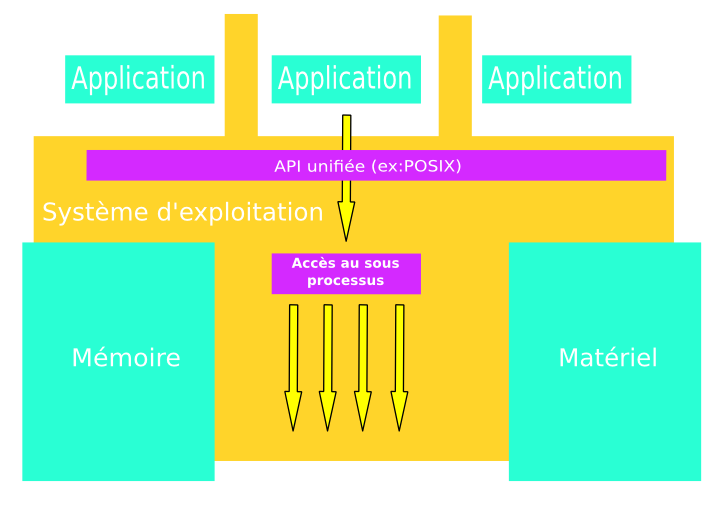
\includegraphics[scale=0.3]{img/operating-system.png}
    \end{center}
  \end{frame}
}

\ifbook{
  \mysubsubsection{Limites physiques d'un ordinateur}
  \paragraph{} Avant d'aller plus loin, arrêtons-nous un instant sur ces notions et sur le système,
  aussi schématique soit-il que nous venons de décrire. Au regard de son fonctionnement, quelles
  limites pouvons-nous déjà percevoir ? Dans quelles conditions, un tel système - l'ordinateur, aura
  des difficultés à effectuer les opérations qu'on lui confie ?

  \paragraph{} Sans surprise, on peut distinguer à peu près autant de limites que de composants
  distingués dans la précédente représentation. Étudions, sommairement, pour chacun d'entre eux les
  limites qu'ils induisent sur l'ordinateur.

  \paragraph{Processeur} La première limite physique d'un ordinateur, qui est pratiquement
  incontournable, est le processeur. Un processeur peut effectuer un certain nombre d'opérations
  dans un certain délai. Dans un système parfaitement optimisé, où tous les autres - assez
  nombreux, nous allons le voir, goulots d'étranglement ont été "neutralisés", cette vitesse
  d'exécution est une limite incompressible : l'ordinateur ne pourra simplement exécuter les
  opérations demandées plus rapidement...

  \paragraph{Parallélisme} Comme évoqué lors de la description du rôle d'un système d'exploitation,
  un ordinateur exécute souvent plusieurs processus à la fois, souvent plus nombreux que son nombre
  de processeurs. Ainsi, il doit passer d'un processus à un autre, à tour de rôle, pour permettre à
  tous de s'exécuter \textit{presque} en parallèle.

  \paragraph{} Il est évident que le passage d'un processus à un autre n'est pas gratuit, et nécessite, de
  la part du système d'exploitation, comme du processeur, un travail supplémentaire qui consiste à
  sauvegarder les données et l'état du processus placé en "pause" et à recharger ceux du processus
  qui "reprend la main".

  \paragraph{} Au bout du compte, si l'ordinateur effectue un nombre de tâches en parallèle
  largement trop grand pour sa capacité, il risque de passer plus de temps à \textbf{changer de
  contexte} entre chaque processus, plutôt qu'à réellement effectuer les opérations qu'on lui
  demande.

  \paragraph{Mémoire} La mémoire à la disposition du processeur impacte généralement grandement la
  vitesse d'exécution. En effet, plus l'ordinateur pourra placer de données en mémoire, plus il
  pourra avoir à sa disposition des résultats intermédiaire et finaux.

  \paragraph{} Illustrons rapidement ce point par un exemple concret. Supposons que l'on confie à
  l'ordinateur de trier un tableau de données, composé d'une seule colonne, par ordre de grandeur
  croissante du contenu de chaque cellule:

  \begin{figure}[h]
    \begin{center}
      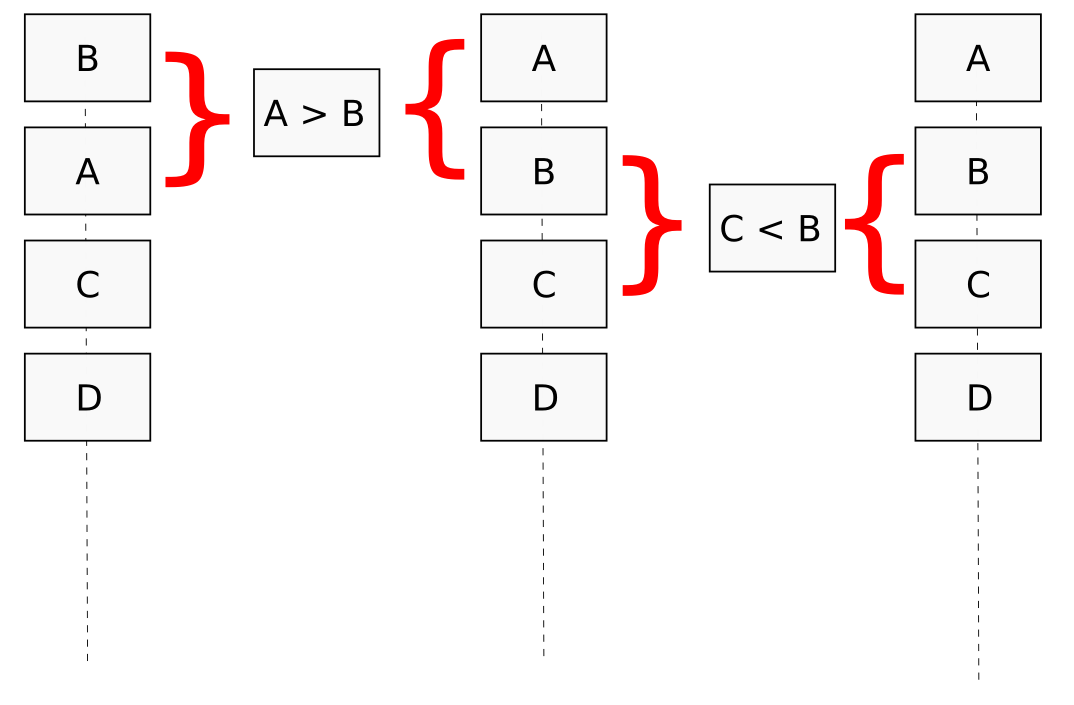
\includegraphics[scale=0.3]{img/exemple-algo.png}
      \caption{Algorithme de tri avec une case mémoire}
      \label{algo-exemple}
    \end{center}
  \end{figure}

}

\ifslide{

  \begin{frame}{Exemple d'algorithme}
    \begin{center}
      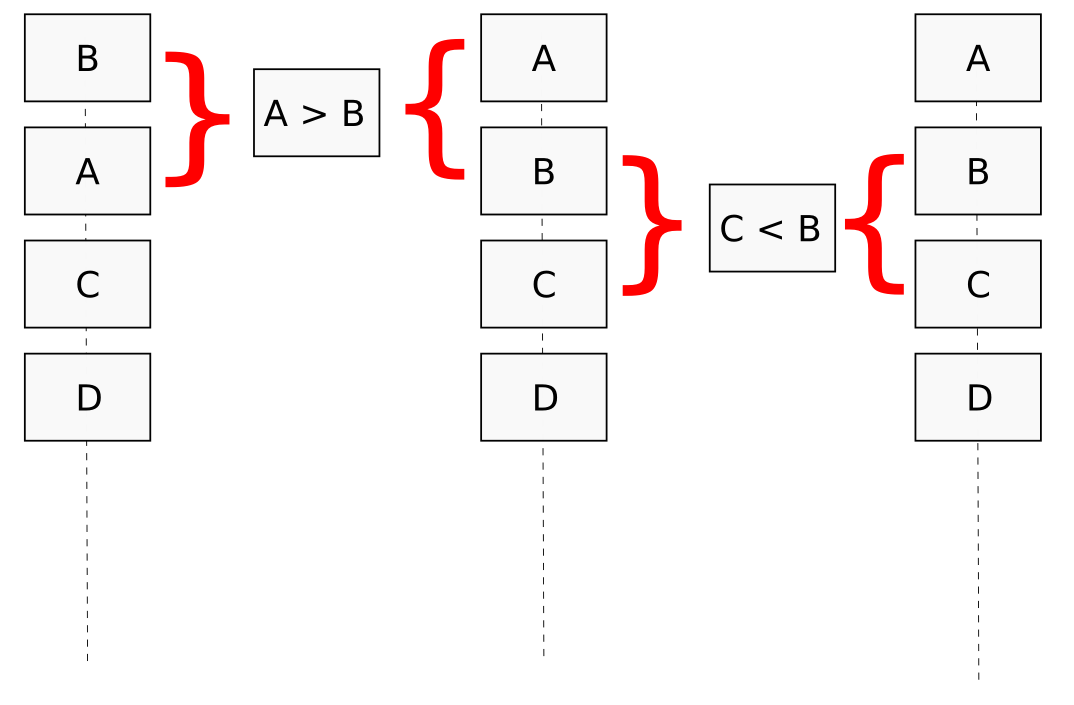
\includegraphics[scale=0.3]{img/exemple-algo.png}
    \end{center}
  \end{frame}
}


\ifbook{

  %TODO:Relire
  \paragraph{} Prenons d'abord comme exemple un ordinateur qui ne pourrait stocker que le contenu
  des quelques cellules du tableau en mémoire rapide. Il devrait alors lire une cellule, lire la
  cellule voisine, les comparer et les réécrire dans le bon ordre. Pour cette opération deux lectures
  et deux écritures ont été nécessaire dans une mémoire lente.

  \paragraph{} Si l'ordinateur avait plus de mémoire alors il aurait pu stocker tout le tableau dans
  sa mémoire la plus rapide, et ainsi réaliser les opérations de lecture beaucoup plus rapidement
  avant d'enfin écrire, en une seule fois, le tableau reclassé dans sa mémoire de stockage de masse,
  elle beaucoup plus lente.

  \paragraph{Remarque} \textit{Cet exemple est volontairement grossier afin de souligner
  l'importance de la mémoire sur la vitesse de traitement.}

  \paragraph{} Si l'ordinateur ne peut stocker qu'un seul résultat intermédiaire, en l'occurrence la
  taille du contenu de la cellule, il ne peut réordonner le tableau qu'en échangeant les cellules
  de positons. En effet, il peut calculer la taille d'une cellule, la stocker, calculer la taille de
  la seconde cellule, la comparer à la précédente et changer l'ordre des deux cellules, si
  nécessaire, puis continuer...

  \paragraph{} Après un laborieux travail, cet \textbf{algorithme}, illustré sur la figure
  \ref{algo-exemple}  (page \pageref{algo-exemple}), sera donc capable de réordonner l'ensemble du
  tableau, mais en effectuant un important nombre d'opérations. À l'inverse, si le processeur est
  libre de placer autant de résultats en mémoire que d'entrées dans le tableau, il pourra se
  contenter de calculer, une fois pour toute, la taille de chaque cellule, puis de les trier de
  manière plus "globale"...

  \paragraph{Remarque} Cet exemple est volontairement très grossier et n'est pas représentatif du
  tout du fonctionnement interne réel d'un ordinateur, ni même de la manière dont le processeur va
  implémenter un algorithme de tri. Néanmoins, sans être l'exemple le plus respectueux des détails
  techniques d'un ordinateur, il illustre de manière très juste l'importance de la mémoire pour la
  réalisation d'opérations au sein d'un ordinateur.

  \paragraph{Entrées/Sorties} Après la mémoire, c'est très certainement les entrées/sorties la
  source de goulot d'étranglement la plus commune au sein d'un ordinateur. Pour bien comprendre
  l'impact de ces dernières sur les performances de l'ordinateur, il suffit de regarder la figure
  \ref{pyramid-io} (page \pageref{pyramid-io} qui décrit, sous forme de pyramide, la vitesse d'accès
  des différentes entrées/sorties, les unes par à rapport aux autres.

  \begin{figure}[h]
    \begin{center}
      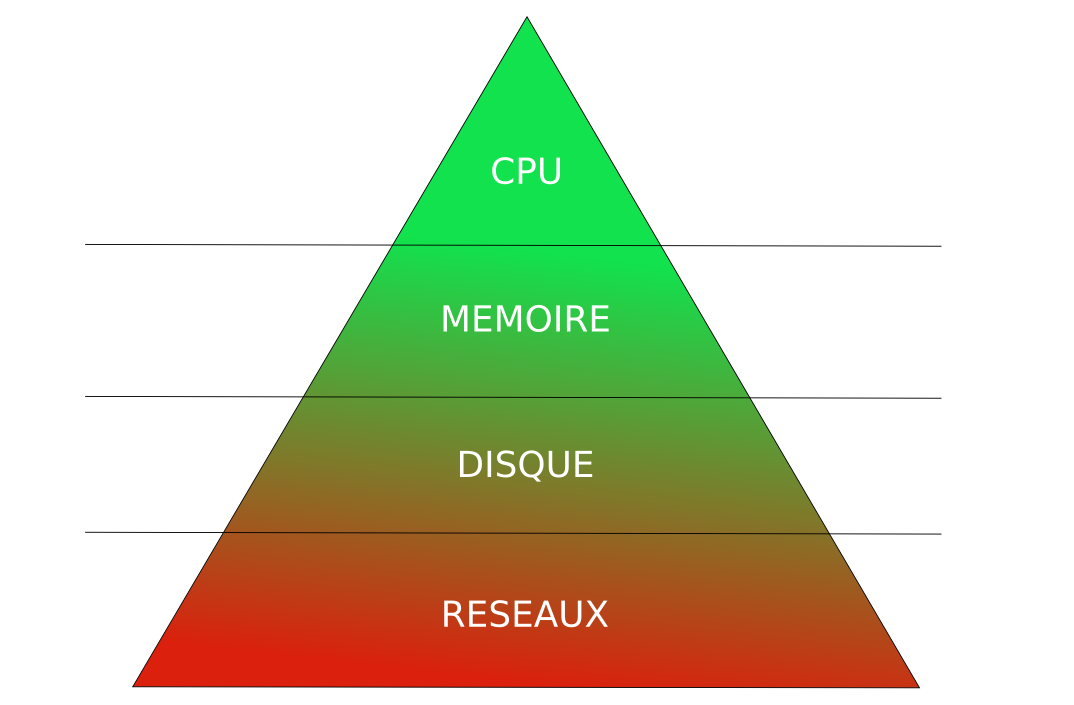
\includegraphics[scale=0.3]{img/pyramid-io.png}
      \caption{Vitesse des entrées/sorties selon les périphériques}
      \label{pyramid-io}
    \end{center}
  \end{figure}

}

\ifslide{
  \begin{frame}{Vitesse d'accès des périphériques}
    \begin{center}
      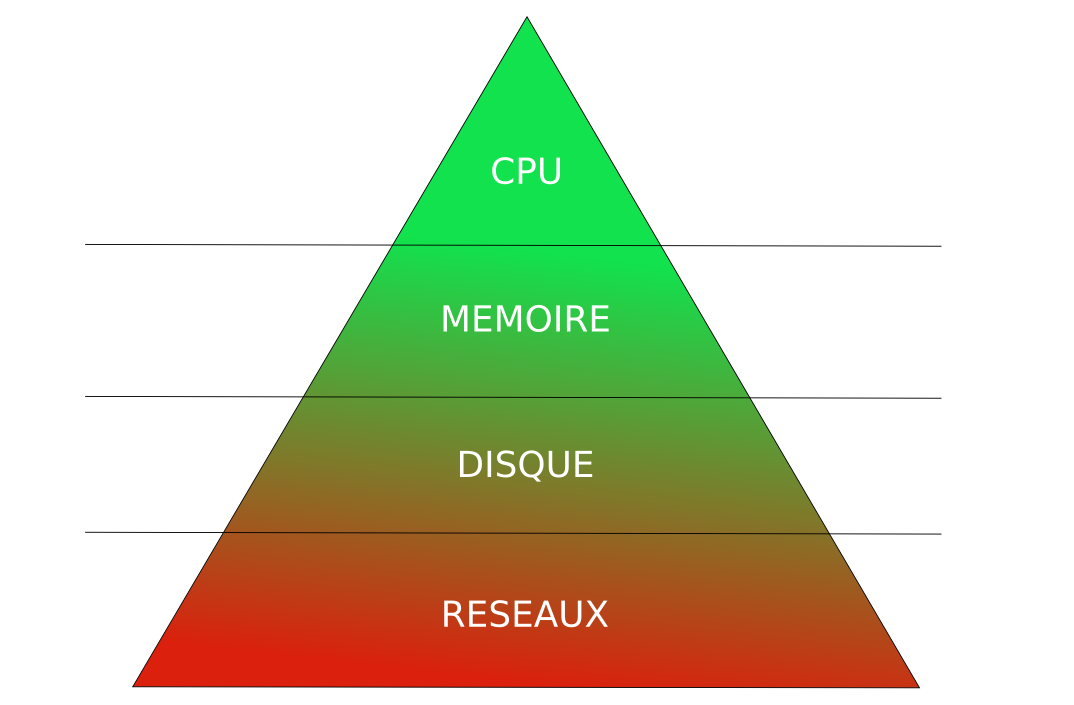
\includegraphics[scale=0.3]{img/pyramid-io.png}
    \end{center}
  \end{frame}
}

\ifbook{

  \paragraph{} À l'étude de ce tableau, il apparaît assez flagrant que si une information nécessaire
  à la bonne exécution du programme est située sur un périphérique inutilement lent (par exemple: sur
  disque dur plutôt qu'en mémoire, sur un serveur distant plutôt que sur le disque dur,...), le
  système en sera ralenti.

  \paragraph{Remarque:} \textit{Ce développement sur les limites physiques d'un ordinateur est volontaire.
  En effet, dans le cadre de la conduite de projet \textit{Middleware}, ces limites seront à
  prendre à compte, dès la conception et l'architecture d'une solution logicielle, pour s'assurer que,
  lors de sa mise en production, le système construit ait une chance de donner les performances
  souhaitées.}

  \paragraph{}\textit{Si des experts techniques sont généralement là pour assister les personnes en charge
  de la conduite, il reste important que ces dernières gardent ses problématiques à l'esprit et soient
  capables d'en discuter avec les susnommés experts...}

}

\subsection{Le modèle client/serveur}

\ifbook{
  \subsubsection{Bref histoire du client léger}
  \paragraph{} Avec l'apparition des réseaux informatiques, apportés par des technologies telles que
  TCP/IP sur laquelle s'est construit le désormais célèbre protocole HTTP, il est rapidement apparu
  très intéressant de pouvoir répartir le traitement sur plusieurs machines.

  \paragraph{} En effet, au début de l'informatique, les machines puissantes coûtaient relativement
  cher, et avaient des capacités de calculs permettant d'effectuer des calculs complexes et de
  répondre aux besoin de nombreux utilisateurs. Ainsi est né le modèle client/serveur, où
  l'utilisateur, à l'aide d'un terminal - une machine peu puissante et peu couteuse, se connecte à
  une machine lui servant des données et exécutant les traitements demandés- un serveur. Le terminal
  se contentant, dans ce modèle, d'afficher le résultat.

  \begin{figure}[h]
    \begin{center}
      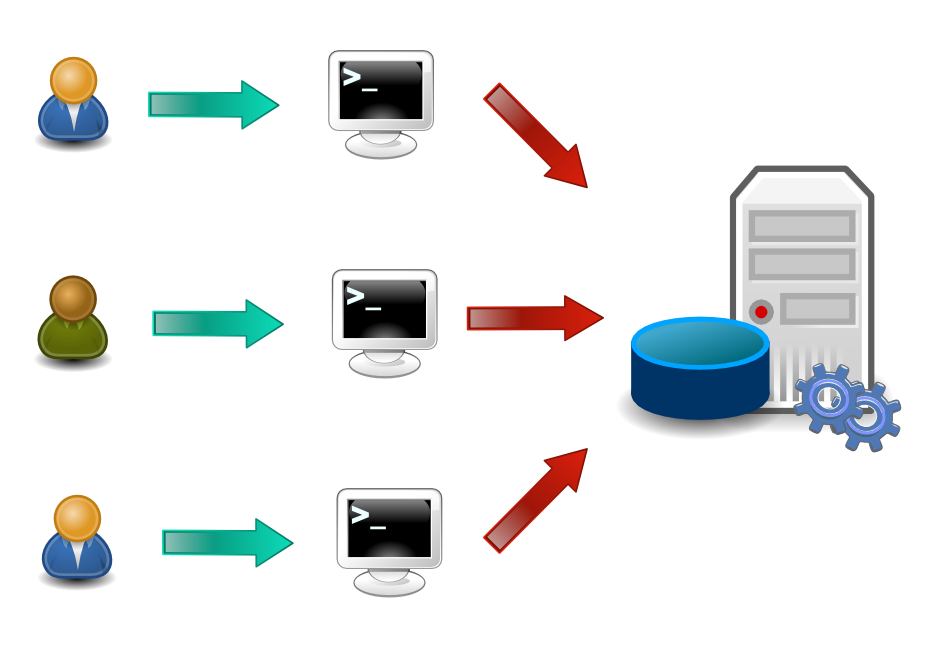
\includegraphics[scale=0.3]{img/mainframe-terminals.png}
      \caption{Terminaux et mainframe}
      \label{mainframe}
    \end{center}
  \end{figure}
}

\ifslide{
  \begin{frame}{Mainframe et terminaux}
    \begin{center}
      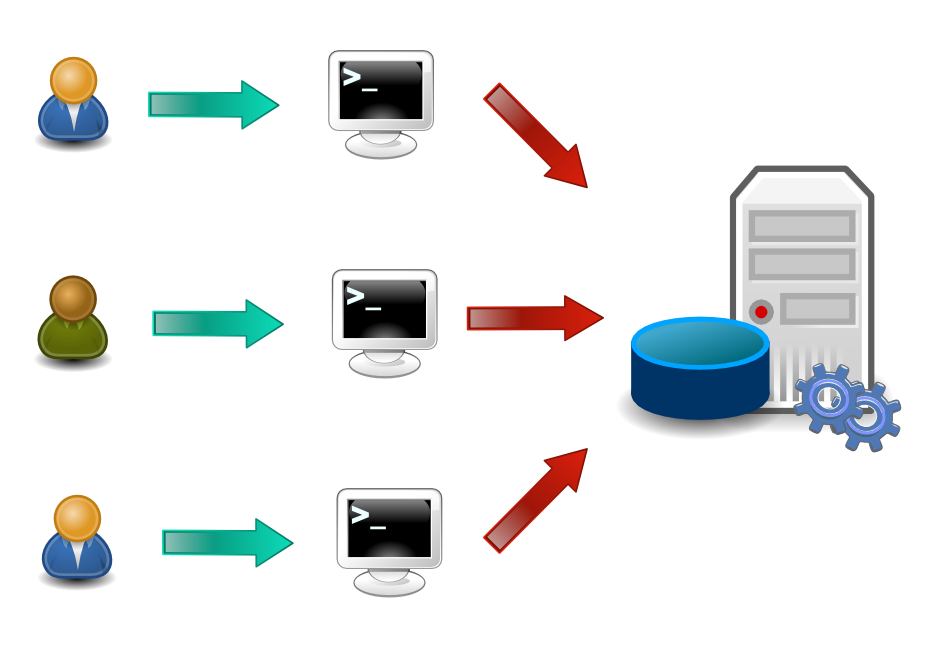
\includegraphics[scale=0.3]{img/mainframe-terminals.png}
    \end{center}
  \end{frame}
}

\ifbook{

  \paragraph{} Avant d'aller plus loin, on peut noter avec intérêt que ce modèle n'est en fin de
  compte pas très différent de celui des débuts d'internet. En effet, à leurs débuts, les
  navigateurs "web" (Mozaic, Netscape, puis Internet Explorer) se contenter simplement d'afficher le
  contenu des pages HTML qu'on leur servaient. Nous y reviendrons par la suite...

  \subsubsection{La naissance du client "lourd"}

  \paragraph{} Ce premier modèle client/serveur se construisait donc sur deux logicielles distincts,
  une première partie s'exécutant sur le terminal de l'utilisateur, le \textbf{client léger}, et une
  seconde partie, plus élaboré et embarquant la \textbf{logique métier} de l'application, le
  \textbf{serveur}.

  \paragraph{Remarque} \textit{L'usage a malheureusement imposé depuis longtemps l'utilisation du même
  terme, \textit{serveur} pour désigner deux entités conceptuellement, mais concrètement
  différentes. Ce terme peut en effet indiquer une machine physique, un ordinateur, relié à un
  réseau informatique et utilisé, à distance, par des utilisateurs, mais le logicielle s'exécutant
  sur ce même type d'ordinateur et fournissant un service applicatfs à ces mêmes utilisateurs.}

  \paragraph{} \textit{La différence est fortement relativement aisée à saisir, mais elle peut tout de même
  porté à confusion. Si dans le cas de la partie précédente nous évoquions la concept de machine
  physique, dans cette section, nous parlons très clairement de \textbf{serveur logicielle}.}

  \paragraph{} Alors que la puissance à la disposition des terminaux augmentaient, et que, dans les
  faits, ceci devinrent des ordinateurs graphiques à usage personnelle ("\textit{Personal Computer
  (PC)}"), il apparu rapidement très pertinent d'en profiter pour offrir des clients plus puissants,
  capable d'effectuer des traitements par eux même, et offrir donc des fonctionnalités
  supplémentaires à leur utilisateurs.

  \paragraph{} Ainsi le mouvement de balancier, qui avait pour but de placer le maximum de logique
  applicatif et de traitement du coté du \textit{serveur}, s'est inversé et les logicielles clients
  devinrent à leur tour de plus en plus complexe, au point qu'on les qualifia de \textbf{clients
  lourds}.

  \begin{figure}[h]
    \begin{center}
      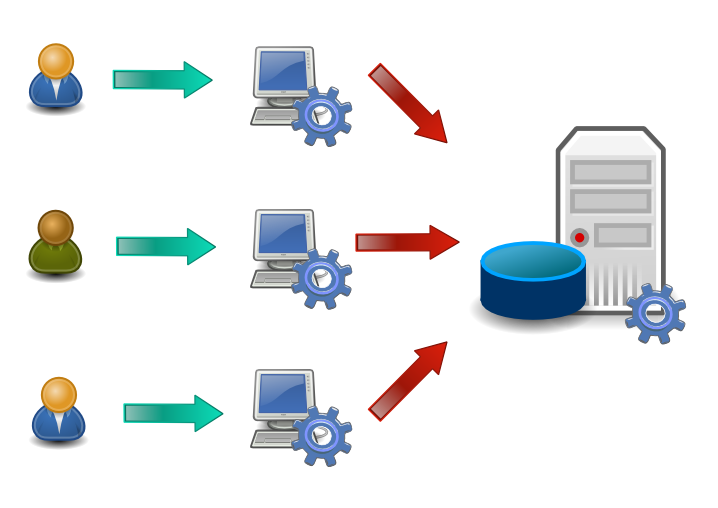
\includegraphics[scale=0.3]{img/fat-clients.png}
      \caption{L'arrivée du PC et des clients lourds}
      \label{fat-clients}
    \end{center}
  \end{figure}

  \subsubsection{Les limites du modèles}

  \paragraph{} Si ce nouvelle déclinaison du modèle aboutit clairement à une manière productivité
  des utilisateurs, du moins dans la plupart des cas, elle posa aussi rapidement des problématiques
  complexes en termes de maintenance. En effet, pour pouvoir faire évoluer le logiciel, il faut
  désormais modifier à la fois le client et à la fois le serveur, et assurer leur rédéploiement
  synchrone. On se retrouva vite malheureusement dans des situations difficiles à gérer, où de
  multiples versions d'une même application clientes sont déployés et doivent cohabiter avec des
  versions différentes de leurs serveurs...
}

\ifslide {
  \begin{frame}{Le modèle client/serveur}
    \begin{center}
      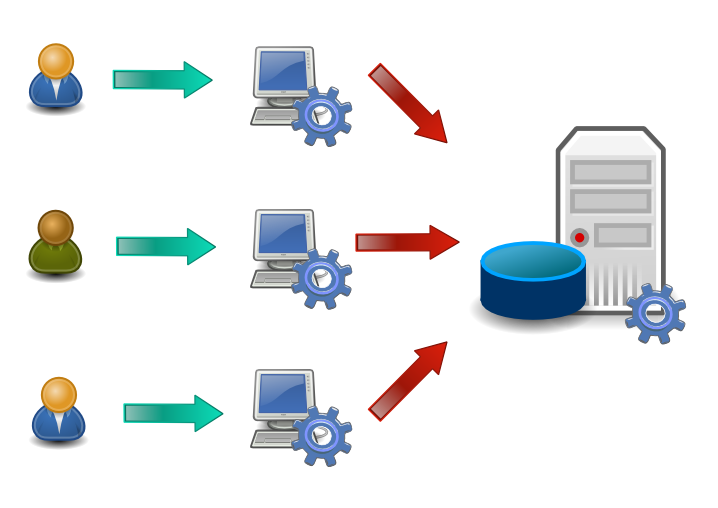
\includegraphics[scale=0.3]{img/fat-clients.png}
    \end{center}
  \end{frame}
}


\ifbook{
  \subsubsection{La Persistance des données: du fichier à la base de données}
  % fichier et répertoires
  \paragraph{} Avant de voir comment les technologies de type client/serveur ont évoluées pour
  circonvenir les problématiques apparues avec l'émergence du client lourd, intéressons nous instant
  non plus au logiciel, mais à ses données, et surtout à leur persistence.

  \paragraph{} Comme évoqué plus haut, un ordinateur travaille avec des données en mémoire et qui
  sont donc par essence, \textbf{volatile}. En effet, lors de l'interruption de l'alimentation de la
  mémoire, les données qu'elle contient sont purement et simplement perdues. Les données n'étant,
  dans la plupart des applications, que rarement dispensable, il a été impératif de trouver des
  mécanismes pour assurer leurs \textbf{persistences}.

  \paragraph{} L'unité atomatique de cette persistence est le \textbf{fichier}. Cette abstraction
  permet de sauvegarder sur une unité de stockage (en langage vernaculaire, un "disque dur") une
  un ensemble d'information de manière séquentielle. On peut retrouver les informations stocké à
  l'aide du nom du fichier.

  \paragraph{} En fait, on peut aisément comparer un fichier à une simple feuille, sur laquelle on
  écrit les données que l'on souhaite persister, un peu de la même manière dont on écrit sur une
  feuille sa liste de courses, pour justement, ne pas l'oublier.

  \paragraph{} Pour permettre de trier et de ranger ses fichiers, dans la prolongation de l'image
  choisi pour les fichiers, des fichiers spéciaux, les \textbf{répertoires} ont été conçu pour
  permettre de aisément ranger et hierarchisé les fichiers.

  \paragraph{} Malheureusement, la manière séquentielle d'organiser les informations d'un fichiers
  se révèla contraignant. En effet, alors que les applications se complexifiaient, et qu'une données
  fit référence à une autre, puis à une autre, la nature \textbf{relationnelle} devint évident et
  imposa un changement de stratégie dans l'approche de leur persistece.

  \paragraph{} En outre, les données nécessite bien souvent d'être partagé entre plusieurs
  applications, et il est fort complexe de partager un fichier de données entre plusieurs
  applicatons. Comment gérer les accès concurrents ? Comment assurer la cohérence des données qui
  sont persisté ?
  % base de donnée
  \paragraph{} Pour palier à ses nombreux problèmes et surtout clairement séparer les données des
  applicatifs, les premières base de données relationelles firent leurs apparitions. En plus de
  permettre de stocker les données hors des applications et de les partager, elles permirent, peu à
  peu, d'établir un langage standard pour interagir avec elles, le SQL (\textit{Standard Query
  Language}).
}

\demoframe{Le SQL}{Argument optionnelle pour le moment}

\ifbook{
  \subsubsection{Architecture n-tiers}
    \paragraph{} Si nous résumons les différents éléments évoqués jusqu'à maintenant sous forme de
    la figure \ref{n-tiers} (page \pageref{n-tiers}), on constate que désormais notre application,
    qui au départ s'exécutait sur une seule machine, relié par un terminal très primaire, est
    désormais réellement éclatée entre plusieurs composant, ou \textbf{tiers}.

    \paragraph{} Ainsi, de l'architecture client/seveur, composé de deux tiers, on est arrivée à une
    architecture 3 tiers, où la base de données vint s'ajouter, en tant que troisième tiers. Mais en
    fait, la séparation des fonctions sur différentes instances physiques a continué, et
    aujourd'hui on parle plus en plus souvent d'architecture \textbf{n-tiers}.

    \begin{figure}[h]
      \begin{center}
        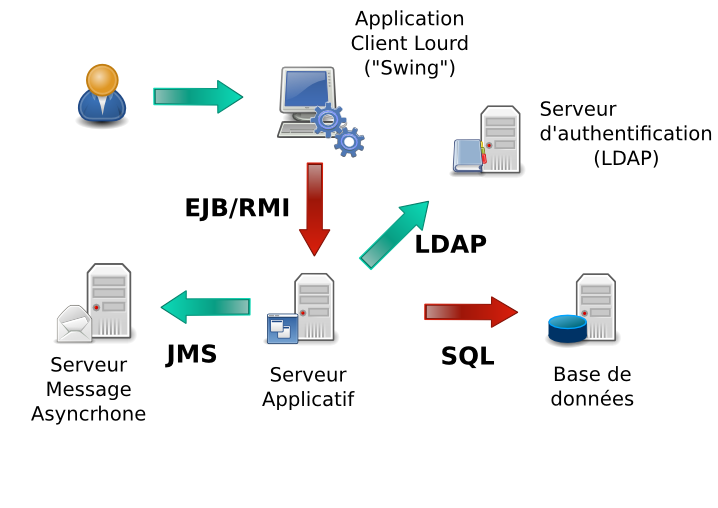
\includegraphics[scale=0.3]{img/n-tiers.png}
        \caption{Exemple d'architecture n-tiers}
        \label{n-tiers}
      \end{center}
    \end{figure}
}

\ifslide{
  \begin{frame}{Architecture n-tiers}
    \begin{center}
      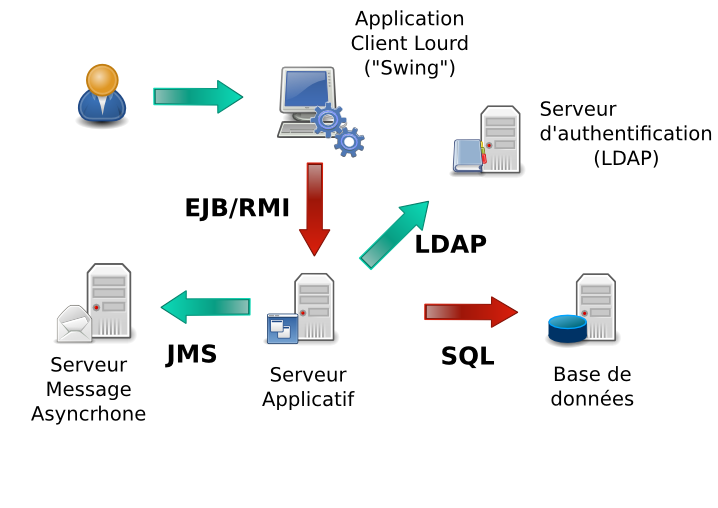
\includegraphics[scale=0.35]{img/n-tiers.png}
    \end{center}
  \end{frame}
}

\ifbook{
  \mysubsubsection{Le Web}
  \paragraph{} Avec l'arrivé des technologies du "Web", soit essentiellement au début, HTML et HTTP,
  le mouvement de balancier évoqué une précédente section s'inverse de nouveau. Dans leurs
  laboratoires, les concepteurs initiale de ce protocole de communication visèrent avant tout la
  simplicitié pour assurer surtout une bonne compatibilité entre les différents systèmes existants
  de part le monde.

  \paragraph{} En effet, avant d'aller plus loin, il est important de se rappeler que à cette
  époque, il existait de nombreux systèmes d'exploitation, tous différents et rarement interopérable
  entre eux. Les plus connues aujourd'hui Apple et Windows, mais à l'époque s'ajouté aussi de
  nombreux types d'Unix différents (cf. \textit{\mylink{http://en.wikipedia.org/wiki/Unix\_wars}{Unix
  Wars}}), accompagné par nombreux autres systèmes, tel que OpenVMS.

  \paragraph{} Sans compter que ces systèmes avaient même des protocoles de communications
  différents. Pour reprendre l'exemple de OpenVMS, ce système utilisé un protocole propriétaire à
  son constructeur, intitulé DecNet et non le standard \textit{de facto} d'aujourd'hui, le protocole
  TCP/IP.

  \paragraph{} Ainsi, concevoir un système applicatif portable - c'est à dire qui fonctionnerait à
  peu près partout et permettrait de communiquer aisément entre des systèmes différents n'était pas
  une simple tâche. C'est donc pour ces raisons, en autres, que les concepteurs de HTTP et de HTML
  ont choisi de faire très simple.

  \paragraph{} Le protocole en lui même est un simple protocole \textbf{texte}, et non binaire, il
  est donc aisé de l'implémenter et, au besoin, de regarder l'échange en lui même pour comprendre la
  source d'un problème. Comme les données échangés sont du texte, tout systèmes de l'époque, aussi
  différent soit-il des autres, était capable de le comprendre.
}

\demoframe{Le protocole HTTP}{
  \begin{block}{Démonstrations}
    \begin{itemize}
      \item simple connection avec telnet
      \item connection complète avec les développeurs tools de Google Chrome
    \end{itemize}
  \end{block}
}

\ifbook{

  \paragraph{} Toujours par souci de simplicité, l'objectif était dans les faits assez peu ambitieux,
  puisqu'il s'agissait d'afficher du contenu simple, du texte un peu enrichi, pour permettre en fait
  au milieu universitaire de publier, facilement et rapidement,  à l'intention de leurs confrères,
  des informations.

  \paragraph{} La conséquence directe de ce choix simple de données utilisés à été de limiter le
  rôle du client à afficher, du mieux possible selon le systèmes utilisées, les informations
  fournies par le serveur HTTP. Le \textbf{client lourd} venait de faire un régime et redevenait un
  \textbf{client léger}.

  % TODO: Dessins de synthèse "web" début
    \begin{figure}[h]
      \begin{center}
        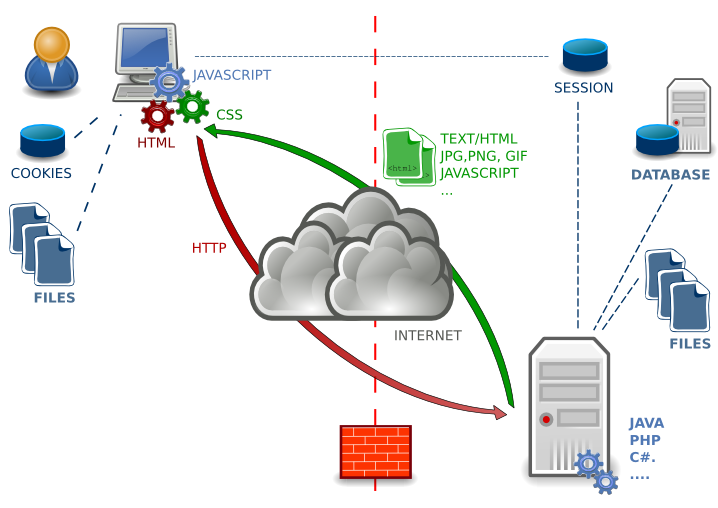
\includegraphics[scale=0.3]{img/internet.png}
        \caption{Extrait de code HTML contenant du Javascript et du CSS}
        \label{internet}
      \end{center}
    \end{figure}
}

\ifslide {
    \begin{frame}{Le "Web"}
      \begin{center}
        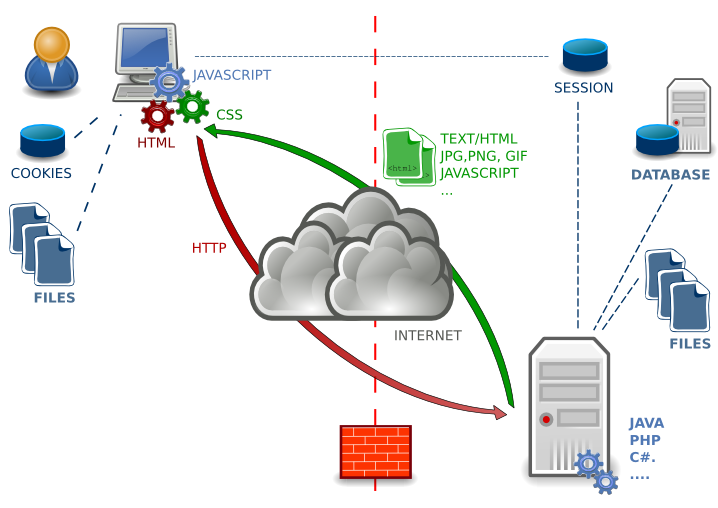
\includegraphics[scale=0.3]{img/internet.png}
      \end{center}
    \end{frame}
}

\ifbook{
  \mysubsubsection{Les technologies "Web" s'enrichissent}
  % Formulaire et session HTTP
  \paragraph{} Le protocole HTTP, et son format de donnée, HTML, a eu le succès qu'on connait, et
  rapidement, malgré l'élégance de la simplicité de la solution, il apparu clair que d'\textbf{absence
  d'interfaction} entre l'utilisateur et le serveur HTTP était une limite trop contraignante. En
  effet, tel que nous l'avons évoqué jusqu'à maintenant, le modèle ne permet en essence que de
  télécharger un page au contenu \textbf{statique}.

  \paragraph{} Pour introduire plus d'interactivité, et permettre au serveur HTTP de modifier
  \textbf{dynamiquement} le contenu des pages présentées selon les demandes des utilisateurs, les
  formulaires ont été introduit. Ces derniers, associés à la méthode HTTP POST, ont donc permis aux
  utilisateurs d'envoyer des données au serveur HTTP, qui furent le point de départ des premières
  applications "web".

  \paragraph{} Mais une fois qu'il fût possible d'envoyer ces données, d'autres limites firent leur
  irruptions. La plupart des applications nécessitant souvent plusieurs échanges entre l'utilisateur
  et le serveur, il fût nécessaire d'ajouter un mécanisme de son coté pour lui permettre de
  conserver les données associées à l'utilisateur, ou plutôt à sa \textbf{session}.

% TODO:Cookies ?
%  \paragraph{} L'ajout donc de la notion de session HTTP permit, là encore, de contourner les limites
%  du modèle original, mais elle ne suffit pas entièrement. De la même manière dont le serveur avait
%  besoin de garder trace de son utilisateur, il fallait aussi que l'on soit en mesure, coté client,
%  de conserver une trace.

  % CSS et Javascript
  \paragraph{} Alors que la première génération de site web finissaient de fleurir, une
  problématique, jusque là invisible, apparu de plus en plus clairement. Le HTML, dans toute la
  beauté de sa simplicité, enfreint par son essence même, une règle pourtant fondamentale de
  l'informatique, que nous avons déjà évoqué avec les bases données : la séparation du contenu et de
  sa présentation.

  \begin{figure}[h]
    \begin{center}
      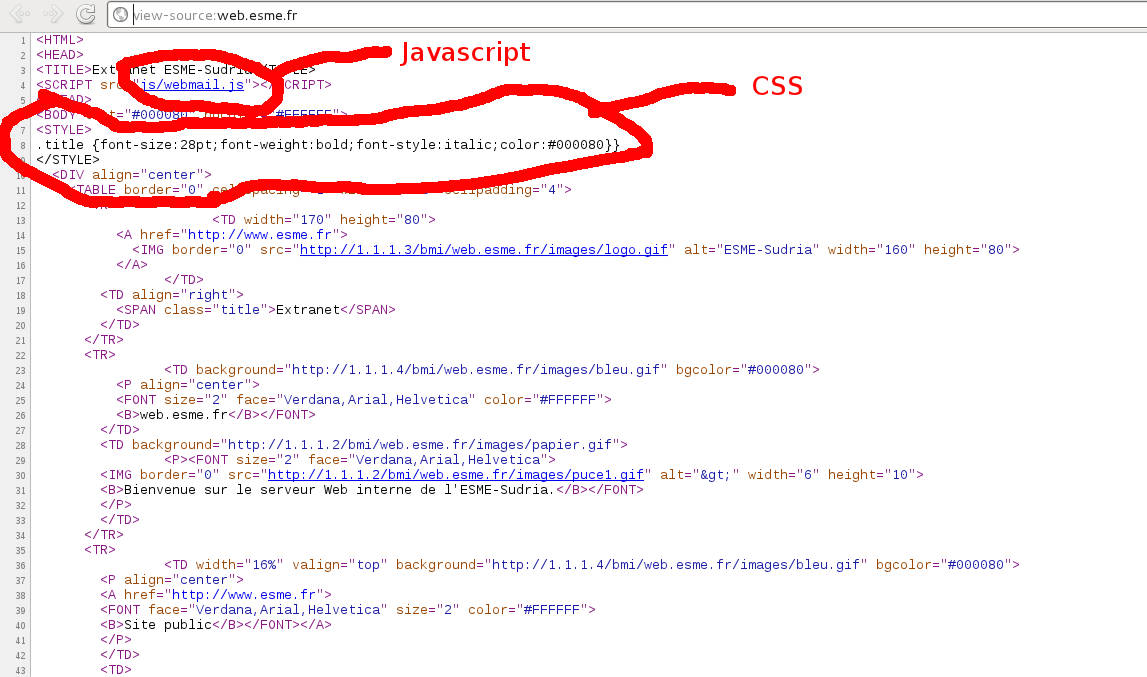
\includegraphics[scale=0.3]{img/html-code-sample.png}
      \caption{Extrait de code HTML contenant du Javascript et du CSS}
      \label{middleware}
    \end{center}
  \end{figure}
}


\ifslide {
  \begin{frame}{HTML, CSS et JavaScript}
    \begin{center}
      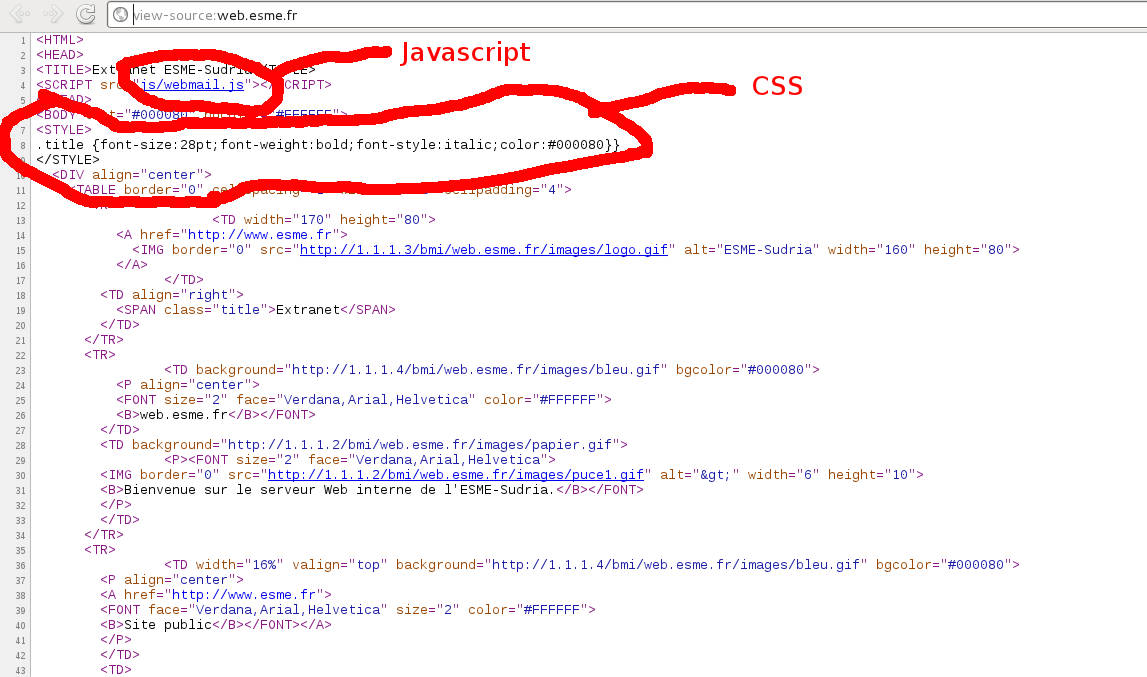
\includegraphics[scale=0.3]{img/html-code-sample.png}
    \end{center}
  \end{frame}
}

\ifbook{
  \paragraph{} En effet, au sein d'une page HTML, on mélange avec allégresse texte avec sa
  présentation qu'il s'agisse de le mettre en gras ou ialic, ou bien de le positionner au sein de la
  page. Et cet état fait rendu rapidement très difficile de faire évoluer, du point fonctionnel, les sites -
  puisque les graphistes ou ergonomes ne pouvait pas travailler de manière indépendantes des
  programmeurs, mais aussi de faire évoluer leurs chartes graphiques, puisque leurs simples mise à
  jour nécessitant de modifier l'intégralité des pages...

  \paragraph{} C'est ainsi que est apparu le CSS, \textit{Cascading Style Sheet}, ou plus
  simplement, les feuilles de styles, dont l'objectif était non seulement de permettre de modifier
  la présentation d'une page HTML existante, mais aussi de séparer la partie présentation d'un site,
  de ses données.

  \paragraph{} En parallèle à l'utilisation du CSS, un autre langage a été introduit, sous forme de
  script, placés dans la page, mais dont l'exécution est déclencheur par le navigareur et qui donc
  fonctionne non plus le serveur, mais sur l poste client.

  \paragraph{} Introduit tout d'abord de manière propriétaire, ce petit langage permis de rendre les
  sites "web" tellement plus dynamique et \textbf{conviviale}, en améliorant grandement
  l'interfaction de l'utilisateur avec ces dernirs, qu'il fût rapidement adopté, et même normalisé
  sous le nom, rarement utilisé, de ECMAScript.
}

\ifbook {
  \mysubsubsection{Conteneur d'exéctution d'application "web"}
  \paragraph{} Comme nous l'avons brièvement résumé, les technologies du "web" se sont construites
  sur une forte volonté d'offrir un système ouvert, standard et interopérable. À l'aide des
  abstractions choisi, et du modèle relativement simple, une page HTML, aussi complexe soit-elle,
  peut être rendu - à peu près, de manière similaire, quelques soit le système d'exploitation
  utilisé.

  \paragraph{} Mais, du coté serveur, les technologies étaient toujours très \textbf{adhérente} à ce
  dernier. Que vous exécutiez sur Apache HTTP, à l'aide du mod CGI, des scripts Shell sous Unix, ou
  que vous écriviez des pages ASP sur un serveur Microsoft, le code réalisé restait indéniablement
  spécifique à son cadre d'exécution.

  \paragraph{} Progressivement, un certain nombres de cadre d'exécution (et de dévelopements)
  d'application "web" virent le jour, tel que PHP et Java. Ces deux derniers, pour continuer avec
  eux, forment des langages de programmation à part entière, mais le modèle qu'ils proposent apporte
  surtout une réelle interopérabilité coté serveur.

  \paragraph{} En effet, avec ce genre de technologie, il devint possible d'exécuter son programme
  sur n'importe quel type de serveur avec un comportement (presque) identique. On pu donc enfin
  aisément migrer de systèmes d'exploitation, dans le cas où celui ci ne se comporte pas de manière
  suffisante pour l'application, ou recruter un développeur sans que celui ci n'est besoin d'autre
  compétences que la seule maitrise de la technologie.

  \paragraph{} En outre, ces technologies promeuvent, pour la plupart, un certain \textbf{modèle de
  programmation}, et l'ecosystème qui les entourent apportent son lot de composants prêt à utiliser
  et destiné à faciliter le développement d'application robuste et capable de monter en charge.

  \begin{figure}[h]
    \begin{center}
      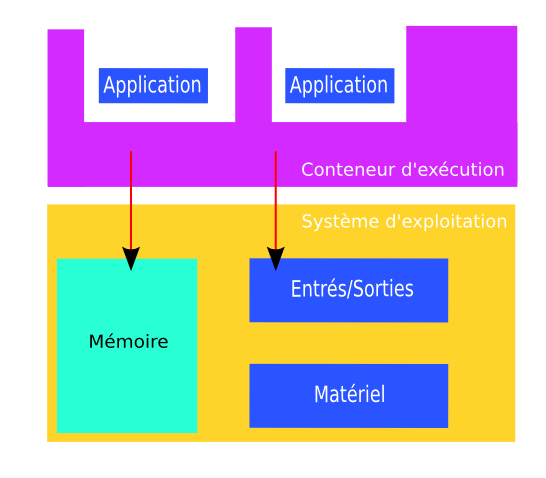
\includegraphics[scale=0.3]{img/execution-container.png}
      \caption{Rôle d'un conteneur d'exécution}
      \label{execution-container}
    \end{center}
  \end{figure}
}


\ifslide {
  \begin{frame}{Conteneur d'exécution}
    \begin{center}
      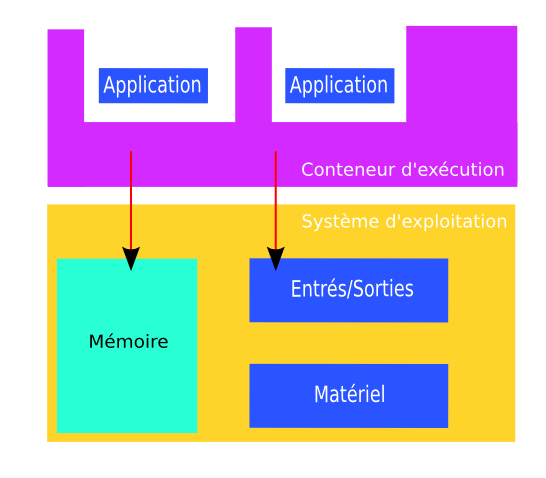
\includegraphics[scale=0.3]{img/execution-container.png}
    \end{center}
  \end{frame}
}

\subsection{Qu'est ce que le middleware ?}

\ifbook {
  \paragraph{} Après ce vaste état des lieux, nous allons enfin pouvoir rentrer dans le thème de ce
  cour: le \textit{Middleware}. En premier lieu, essayons de trouver une définition un plus parlante
  de ce terme, qui n'est pas réellement de traduction française.

  \paragraph{} Si on on traduit très littéralement ce terme, on obtient quelques chose de l'ordre du
  "matériel du milieu". Bon, c'est peu parlant, mais clairement le suffix "\textit{-ware}" fait echo
  aux termes \textit{"software"} - le matériel logiciel, et \textit{"hardware"}, le matériel
  physique, ce qui signifie que, en fait, le mot clé ici, est le "milieu".

  \paragraph{} Mais de quoi exactement sommes nous au milieu ici ? Revoyons simplement notre dessin
  d'architecture à n-tiers:

  \begin{figure}[h]
    \begin{center}
      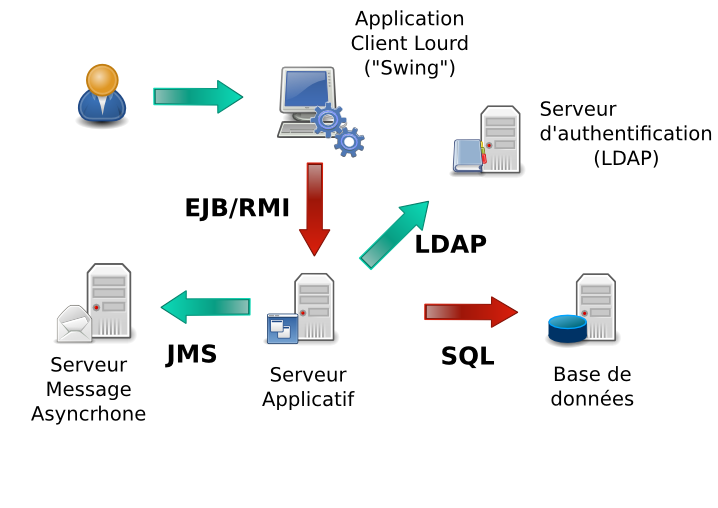
\includegraphics[scale=0.3]{img/n-tiers.png}
      \caption{Où se trouve le middleware sur cette figure ?}
      \label{where-is-middleware}
    \end{center}
  \end{figure}
}

\ifslide{
   \begin{frame}{Qu'est ce que le middleware ?}
     \begin{center}
       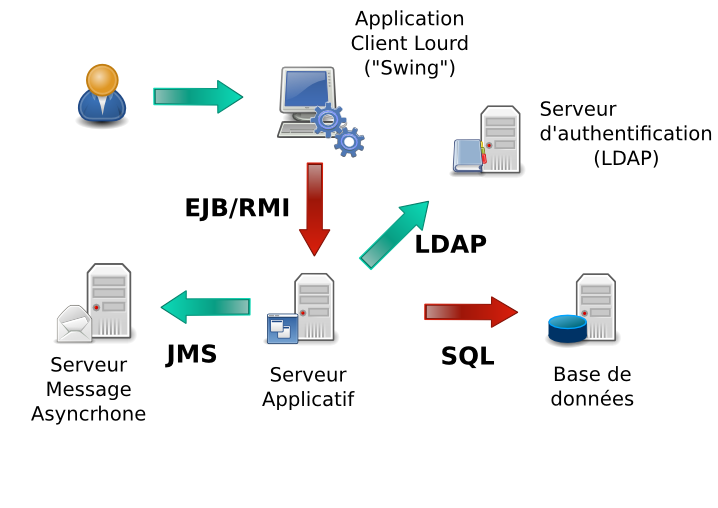
\includegraphics[scale=0.35]{img/n-tiers.png}
     \end{center}
   \end{frame}
}

\ifbook{

  \paragraph{} Le \textit{Middleware} est tout simplement ce qui se retrouve, littéralement, au
  milieu ! Soit entre la base de données et les clients utilisées par les usagers du système. Mais
  au milieu, il y a l'application, non ? Certes oui, mais, celle ci ne s'appuye désormais plus sur les
  seules API fournies par le système d'exploitation, mais sur une kyrielle de services. Ces derniers
  proviennent soit de son environnement d'exécution - tel que une machine virtuelle comme celle de
  Java ou C\#, ou un serveur d'application, ou encore par des composants que l'application elle-même
  embarque.

  \paragraph{} Mais qu'apportent ces services de plus ? Nous allons étudier le "catalogue" en
  détails durant ce cours, mais en quelques mots, ils apportent beaucoup ! Gestion de \textit{pool}
  de connexion, cache locale ou distribué, sécurité, intégration avec un service d'authentification
  distant ou même encore la capacité de mettre en \textit{cluster} l'application pour assurer
  aisément sa montée en charge simplement en ajoutant de nouvelles machines.

  \paragraph{} Pour en revenir à une sorte de définition du \textit{Middleware}, nous retiendrons
  donc que ce dernier est l'ensemble des services utilisées par l'application, aussi bien en son
  sein, que pour communiquer avec des services distants. Bref, en essence, le \textit{Middleware} se
  trouve bel et bien "au milieu", entre l'application et le reste du monde...

  \paragraph{} En essence, le \textit{Middleware}, c'est les briques avec lesquelles on construit
  l'application métier que l'on souhaite réaliser.
  % TODO: dessin fin de déf du middleware ? (img rigolote ?)
}

\subsection{Caractéristiques de la Programmation Orienté Objet}

\newcommand{\bizProcessExemple}[0]{
  \begin{enumerate}
    \item créer un nouveau salarié dans la base de données
    \item ajouter la salarié dans l'équipe de son manager
    \item notifier par email les membres de l'équipe de l'arrivée du nouveau membre
  \end{enumerate}
}

\ifbook{

  \paragraph{} La paradigme de la programmation orienté objet se retrouve dans  plusieurs
  problématiques liées au \textbf{Middleware}, il est important d'expliciter quelques unes de ses
  caractéristiques.

  \subsubsection{Programmation impérative}

  \paragraph{} La paradigme de la programmation orienté objet se retrouve dans  plusieurs
  problématiques liées au \textbf{Middleware}, il est important d'expliciter quelques unes de ses
  caractéristiques.

  \paragraph{} En premier lieu, il faut savoir que la programmation orienté object se définit
  essentiellement par sa distinction avec la programmation \textbf{procédurale} ou
  \textbf{impérative}. Dans ce style de programmation, on effectue les traitements les uns à la suite
  des autres, en regroupant le code commun dans des fonctions.

  \paragraph{} Prenons l'exemple de traitement procédurale:

  \bizProcessExemple

  \paragraph{} Une approche impérative consisterait ici à réaliser un programme réalisant chacune de
  ces actions, dans l'ordres. C'est une approche tout à fait valide et elle ne pose pas, en soi, de
  problème.

  \subsubsection{Approche par "objet"}

  \paragraph{} Néanmoins, la programmation orienté objet propose une approche, qui apporte de nombreux
  avantages. Cette approche consiste à ne plus se concentrer sur la séquence de traitement à réaliser,
  mais plutôt sur les données utilisées.

  \paragraph{} En effet, le but du jeu ici est d'\textbf{encapsuler} les données dans des objets, et
  ne le laisse le reste du programme interagir avec ces données que par le biais des fonctions
  qu'elles proposent. Ces fonctiones se nomment en fait désormais des \textbf{méthodes}.

  \paragraph{} L'objectif de ceci est de \textbf{masquer} la nature réelle des données, et de
  n'exposer que les traitements disponibles autour de ces données. Ainsi, si la nature des données ou
  même des détails d'implémentations des traitements proposés venaient à changer, ces modifications
  seront transparente pour le reste du programme.
}

\ifslide {
  \subsection{Programmation impérative versus programmation orienté objet}
  \begin{frame}
    \begin{block}{Ajout d'un nouvel employé}
      \bizProcessExemple
    \end{block}
    \begin{center}
      
\includegraphics[scale=0.30]{img/biz-process-banner.png}
    \end{center}
  \end{frame}
}

\ifbook{

  \paragraph{} Illustrons ce point en reprenant notre exemple précédent. Pour implémenter notre
  processus métier - l'ajout d'un nouveau employé dans une équipe, nous allons désormais définir
  plusieurs \textbf{objet}.

  \paragraph{} Le premier objet sera l'objet salarié. Ce dernier résultura de la création du salarié
  dans la base de données de l'entreprise, et il regroupe l'ensemble des données relatives à un
  employé. L'accès à la base de données des salariés sera aussi un objet.

  \paragraph{} Le second objet sera en fait une collection de salarié que forme son équipe. Pour
  réaliser le second point de notre traitement, il suffira donc d'ajouter le salarié créée juste avant
  à la liste des salariés composant l'équipe.

  \paragraph{} Un autre objet sera en charge de l'envoi des mails, et sera donc utilisé pour notifier
  les différents membres de l'équipe de l'arrivée du nouveau membre de l'équipe.
}

\ifslide{
  \begin{frame}
    \begin{center}
      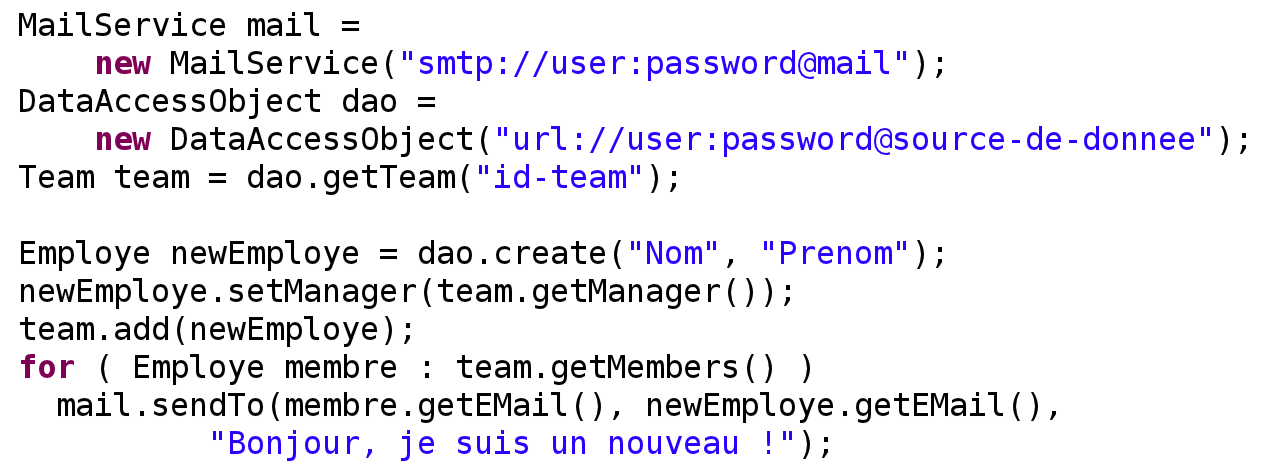
\includegraphics[scale=0.25]{img/biz-process-code-sample.png}
    \end{center}
  \end{frame}
}

\ifbook{

  \begin{figure}[h]
    \begin{center}
      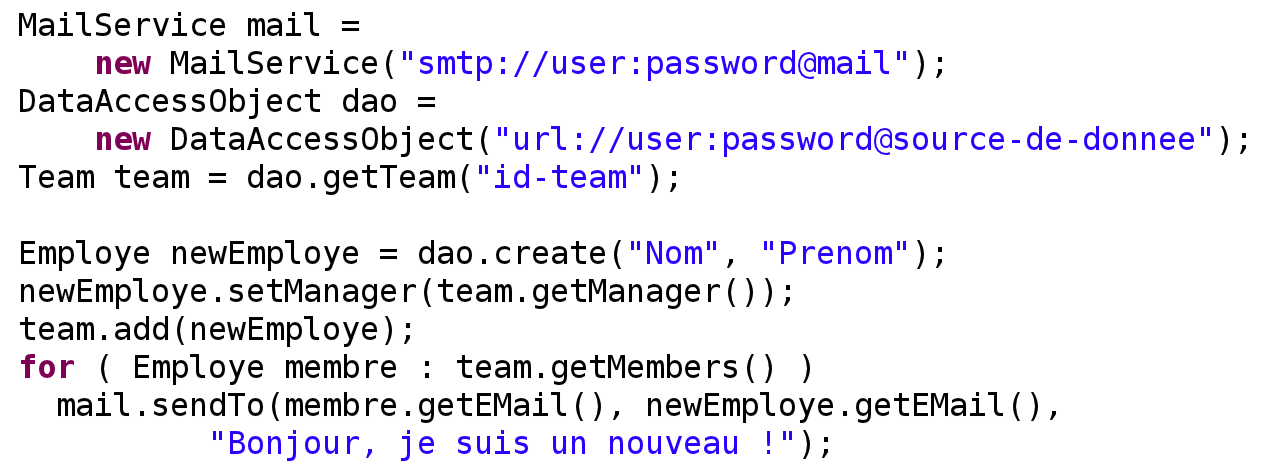
\includegraphics[scale=0.35]{img/biz-process-code-sample.png}
      \caption{Exemple de code orienté objet}
      \label{biz-process-code}
    \end{center}
  \end{figure}

  \paragraph{} Comme l'illustre l'extrait de code \ref{biz-process-code} (page
  \pageref{biz-process-code}, ce style de programmation qu'est la  programmation orienté objet
  permet d'obtenir un code très simple et lisible, mais surtout facilement réutilisable. Par
  exemple, l'objet DataAccessObject regroupe tout le code nécessaire pour se connecter à la base de
  données. Il suffit de réutiliser cet objet, ailleurs dans le code du programme si l'on souhaite
  effectuer des opérations avec la base de données.

  \paragraph{} Un autre avantage immédiat de cette approche est de pouvoir concevoir aisément des
  objets "métiers" décrivant de manière isolé et unitaire, les différents traitements spécifique au
  métier de l'entreprise ou l'organisation. Les différents applications pourront ensuite aisément
  s'appuyer sur ces bibliothèques d'objets pour réaliser les différents traitements qui leur sont
  spécifiques.
}

%- dessin "application" => "pile, gestion de threads, cache, ...", puis vers le modèle java/jee de container
%- évoqué la problématique du packaging et de la réutilisation de code, probablématique de gestion de version aussi

% expliciter/décrire le besoin, dans la conception d'un IT, de découper son "business" en module,
% d'avoir est du code partagé (des Jars) mais aussi des applicatifs qui utilisent les mêmes briques,
% les mêmes services, etc...


\section{B - Les services applicatifs 1/2 (10/01/2012)}

\abstractframe{Ciblé sur application, ce chapitre du cours se concentre
sur les services et composants proposés par les \textit{middlewares} à cette
dernière}{../img/overview-services.png}

\subsection{Serveur d'applications}
\subsubsection{Pool(s) de connexion}
\subsubsection{Threads}

\subsection{Conteneur Web}
\subsubsection{Connecteur HTTP et Servlet}
\subsubsection{Session et Cookie}

\subsection{Transaction}

\subsection{Cache}

\section{B - Les services applicatifs 2/2 (10/01/2012)}
\subsection{Gestion des processus métiers (BPM)}

\subsection{Message et communication asynchrone}

\subsection{Sécurité}
% \begin{frame}
%   \begin{itemize}
%   \item Gestion d'identité (SSO, Annuaire,...)
%   \item Modèle de Sécurité (EJB, JAAS)
%   \end{itemize}
% \end{frame}
\subsection{Modèle de programmation}
% \begin{frame}
%   \begin{itemize}
%     \item gestion de l'état
%     \item concurrence
%   \end{itemize}
% \end{frame}

\section{C - Application distribuée et intégration (11/01/2012)}
\abstractframe{Élargissant le spectre au-delà du périmètre de l'application,
cette partie étudie les services et composants proposés par les
\textit{middlewares} pour dialoguer, et s'intégrer, à son environnement, et plus
spécialement à la nature \textbf{distribuée} du système d'information dans lequel
elle évolue.}{../img/overview-integration.png}

\subsection{Source de données}

\subsubsection{Fichiers et ressources}
\subsubsection{SQL et base de données relationnelle}
\subsubsection{Annuaire}
\subsubsection{NoSQL}
\subsection{Programmation distribuée}
% \begin{block}{Historique}
%   \begin{itemize}
%     \item RPC
%     \item CORBA
%     \item Java-RMI
%     \item DCE
%     \item COM/DCOM
%   \end{itemize}
% \end{block}
\subsection{Transaction distribuée}
\subsection{Architecture orientée service (SOA)}
\subsubsection{WebServices}
%   \begin{itemize}
%     \item SOAP et WSDL
%     \item ReST
%   \end{itemize}

\subsubsection{Bus logiciel (ESB)}
\subsection{ETL, EAI et autres middlewares}

\section{D - Mise à échelle et production (12/01/2012)}

\subsection{Problématique de performances des middlewares}

\subsection{Stratégie de mise à l'échelle (Ferme, clustering...)}

\subsection{Indicateur, surveillance et alertes}

\abstractframe{Cette partie évoque les problématiques liées à la mise en production
et la surveillance d'une application et des \textit{middlewares} qu'elle
utilise.}{../img/overview-monitoring.png}


